\begin{tomtat}
	\begin{minipage}[t]{0.3\textwidth}
		\vspace{0pt}
		\begin{tomtat}
			\begin{center}
				\textbf{ĐỀ 16}
			\end{center}
			
		\end{tomtat}
	\end{minipage}
	\hfill
	\begin{minipage}[t]{0.5\textwidth}
		\vspace{0pt}
		\begin{tomtat}
			\begin{center}
				\includegraphics[scale=0.08]{images/16}
			\end{center}
		\end{tomtat}
	\end{minipage}
\end{tomtat}
\textbf{I. PHẦN TRẮC NGHIỆM}
\begin{ex} % Câu 1
	Nghiệm của phương trình: $4(x-2)-(x-1)=0$ là:
	\choice{$x=2$ và $x=1$}{$x=\frac{7}{3}$}{$x=\frac{9}{5}$}{$x=2$ hoặc $x=1$}
	\loigiai{
		Ta giải phương trình:
		\begin{align*}
			4(x-2)-(x-1) &= 0 \\
			4x - 8 - x + 1 &= 0 \\
			(4x-x) + (-8+1) &= 0 \\
			3x - 7 &= 0 \\
			3x &= 7 \\
			x &= \frac{7}{3}
		\end{align*}
		Vậy nghiệm của phương trình là $x=\frac{7}{3}$.
		\\ \textbf{ĐÁP ÁN B}
	}
\end{ex}

\begin{ex} % Câu 2
	Nghiệm của bất phương trình: $-4x+2<0$ là:
	\choice{$x<\frac{1}{2}$}{$x>\frac{1}{2}$}{$x>2$}{$x<2$}
	\loigiai{
		Ta giải bất phương trình:
		\begin{align*}
			-4x+2 &< 0 \\
			-4x &< -2
		\end{align*}
		Khi chia cả hai vế của bất phương trình cho một số âm (ở đây là -4), ta phải đổi chiều bất đẳng thức:
		\begin{align*}
			x &> \frac{-2}{-4} \\
			x &> \frac{1}{2}
		\end{align*}
		Vậy nghiệm của bất phương trình là $x>\frac{1}{2}$.
		\\ \textbf{ĐÁP ÁN B}
	}
\end{ex}

\begin{ex} % Câu 3
	Tính giá trị của biểu thức: $\sqrt{75}+\sqrt{12}$
	\choice{$3\sqrt{3}$}{$10\sqrt{3}$}{$7\sqrt{3}$}{$5\sqrt{3}$}
	\loigiai{
		Ta có:
		\begin{align*}
			\sqrt{75}+\sqrt{12} &= \sqrt{25 \cdot 3} + \sqrt{4 \cdot 3} \\
			&= 5\sqrt{3} + 2\sqrt{3} \\
			&= (5+2)\sqrt{3} \\
			&= 7\sqrt{3}
		\end{align*}
		\\ \textbf{ĐÁP ÁN C}
	}
\end{ex}

\begin{ex} % Câu 4
	Cho tam giác ABC vuông tại B, có AB=5cm, BC=10cm. Khi đó $\tan C$ bằng:
	\choice{$\frac{1}{2}$}{$\frac{1}{3}$}{$\frac{1}{4}$}{$\frac{1}{5}$}
	\loigiai{
		Trong tam giác ABC vuông tại B:
		Theo định nghĩa tỉ số lượng giác tang, ta có:
		$$ \tan C = \frac{\text{cạnh đối}}{\text{cạnh kề}} = \frac{AB}{BC} $$
		Với $AB=5 \text{ cm}$ và $BC=10 \text{ cm}$, ta có:
		$$ \tan C = \frac{5}{10} = \frac{1}{2} $$
		\\ \textbf{ĐÁP ÁN A}
	}
\end{ex}

\begin{ex} % Câu 5
	Cho $(O;6\text{cm})$, trên đường tròn lấy hai điểm M và N sao cho $\widehat{MON}=120^\circ$. Độ dài cung nhỏ MN là: (lấy $\pi \approx 3,14$)
	\choice{$25,12\text{cm}^2$}{$3,14 \text{ cm}^2$}{$6,28\text{cm}^2$}{$12,56\text{cm}^2$}
	% Lưu ý: Đơn vị của độ dài cung phải là cm, không phải cm^2. Các đáp án có vẻ nhầm đơn vị.
	\loigiai{
		Độ dài cung tròn được tính bằng công thức: $l = \frac{\pi R n}{180}$.
		Trong đó $R$ là bán kính đường tròn ($R=6 \text{ cm}$) và $n$ là số đo góc ở tâm chắn cung đó ($n=120^\circ$).
		Sử dụng $\pi \approx 3,14$.
		\begin{align*}
			l_{MN} &= \frac{3,14 \cdot 6 \cdot 120}{180} \\
			&= \frac{3,14 \cdot 6 \cdot 2}{3} \\
			&= 3,14 \cdot 2 \cdot 2 \\
			&= 3,14 \cdot 4 \\
			&= 12,56 (\text{cm})
		\end{align*}
		Nếu các đáp án đều là diện tích (cm$^2$), thì có thể đề bài hỏi diện tích hình quạt.
		Diện tích hình quạt: $S_q = \frac{\pi R^2 n}{360} = \frac{3,14 \cdot 6^2 \cdot 120}{360} = \frac{3,14 \cdot 36 \cdot 1}{3} = 3,14 \cdot 12 = 37,68 \text{ cm}^2$.
		Tuy nhiên, câu hỏi rõ ràng là "Độ dài cung nhỏ MN".
		Vậy độ dài cung nhỏ MN là $12,56 \text{ cm}$. Đáp án D có giá trị đúng nhưng đơn vị sai.
		\\ \textbf{ĐÁP ÁN D} (Coi như đơn vị là cm)
	}
\end{ex}

\begin{ex} % Câu 6
	Cho bảng tần số điểm kiểm tra giữa kỳ II môn toán của 25 học sinh lớp 9A như sau:
	\begin{center}
		\begin{tabular}{|l|c|c|c|c|c|c|c|c|c|}
			\hline
			Điểm & 2 & 3 & 4 & 5 & 6 & 7 & 8 & 9 & 10 \\
			\hline
			Tần số & 1 & 1 & 1 & 2 & 4 & 3 & 4 & 6 & 3 \\
			\hline
		\end{tabular}
	\end{center}
	Tần số tương đối của giá trị 8 điểm là:
	\choice{16\%}{50\%}{32\%}{21\%}
	\loigiai{
		Tổng số học sinh (kích thước mẫu) là $N = 25$.
		Tần số của giá trị 8 điểm là $n_8 = 4$.
		Tần số tương đối của giá trị 8 điểm được tính bằng công thức: $f_8 = \frac{n_8}{N} \times 100\%$.
		$$ f_8 = \frac{4}{25} \times 100\% $$
		$$ f_8 = 0,16 \times 100\% = 16\% $$
		\\ \textbf{ĐÁP ÁN A}
	}
\end{ex}
\begin{ex}
	Cho phương trình $2x^2+x-1=0$ có tập nghiệm là:
	\choice{$\{-1; \frac{1}{2}\}$}{$-\frac{1}{2}; 1$}{$\{-1\}$}{$\emptyset$}
	\loigiai{
		Phương trình $2x^2+x-1=0$ là phương trình bậc hai có dạng $ax^2+bx+c=0$ với $a=2$, $b=1$, $c=-1$.
		Ta tính biệt thức $\Delta = b^2-4ac = 1^2 - 4(2)(-1) = 1 + 8 = 9$.
		Vì $\Delta > 0$ nên phương trình có hai nghiệm phân biệt:
		$x_1 = \frac{-b + \sqrt{\Delta}}{2a} = \frac{-1 + \sqrt{9}}{2(2)} = \frac{-1+3}{4} = \frac{2}{4} = \frac{1}{2}$.
		$x_2 = \frac{-b - \sqrt{\Delta}}{2a} = \frac{-1 - \sqrt{9}}{2(2)} = \frac{-1-3}{4} = \frac{-4}{4} = -1$.
		Vậy tập nghiệm của phương trình là $S = \{-1; \frac{1}{2}\}$.\\
		\textbf{ĐÁP ÁN A}
	}
\end{ex}


\begin{ex} % Câu 8
	Một hình nón có đường kính đáy là 2cm, chiều cao là 9cm. Tính thể tích hình nón đó (lấy $\pi \approx 3,14$, làm tròn đến hàng phần mười).
	\choice{$37,68\text{cm}^3$}{$37,7\text{cm}^3$}{$37,6\text{cm}^3$}{$37,69\text{cm}^3$}
	\loigiai{
		Đường kính đáy của hình nón là $d = 2 \text{ cm}$, vậy bán kính đáy là $R = \frac{d}{2} = \frac{2}{2} = 1 \text{ cm}$.
		Chiều cao của hình nón là $h = 9 \text{ cm}$.
		Thể tích của hình nón được tính bằng công thức: $V = \frac{1}{3}\pi R^2 h$.
		Sử dụng $\pi \approx 3,14$.
		\begin{align*}
			V &= \frac{1}{3} \times 3,14 \times (1)^2 \times 9 \\
			&= \frac{1}{3} \times 3,14 \times 1 \times 9 \\
			&= 3,14 \times \frac{9}{3} \\
			&= 3,14 \times 3 \\
			&= 9,42 (\text{cm}^3)
		\end{align*}
		Làm tròn kết quả đến hàng phần mười, ta được $9,4 \text{ cm}^3$.
		
		% Lưu ý: Các đáp án A, B, C, D có vẻ không khớp với kết quả tính toán. 
		% Kiểm tra lại đề bài hoặc các đáp án.
		% Nếu đường kính là 4cm (R=2cm) thì:
		% V = 1/3 * 3.14 * (2)^2 * 9 = 1/3 * 3.14 * 4 * 9 = 3.14 * 4 * 3 = 3.14 * 12 = 37.68 cm^3.
		% Trong trường hợp này, đáp án A sẽ đúng.
		% Giả sử đề có R=2cm (đường kính 4cm) thay vì đường kính 2cm.
		
		Nếu giả sử đường kính đáy là $4\text{cm}$ (tức là bán kính $R=2\text{cm}$), thì:
		\begin{align*}
			V &= \frac{1}{3} \times 3,14 \times (2)^2 \times 9 \\
			&= \frac{1}{3} \times 3,14 \times 4 \times 9 \\
			&= 3,14 \times 4 \times 3 \\
			&= 3,14 \times 12 \\
			&= 37,68 (\text{cm}^3)
		\end{align*}
		Làm tròn đến hàng phần mười: $37,7 \text{ cm}^3$.
		\\ \textbf{ĐÁP ÁN B} (Với giả định đường kính đáy là 4cm, bán kính là 2cm)
	}
\end{ex}
\textbf{II. PHẦN TỰ LUẬN}
\begin{ex} % Câu 9 (Rút gọn)
	Cho $x \ge 0, x \ne 9$. Rút gọn: $A=\frac{1}{3-\sqrt{x}}+\frac{1}{\sqrt{x}+3}+\frac{2\sqrt{x}}{x-9}$.
	\loigiai{
		Với $x \ge 0, x \ne 9$, ta có $x-9 = (\sqrt{x}-3)(\sqrt{x}+3) = - (3-\sqrt{x})(\sqrt{x}+3)$.
		\begin{align*}
			A &= \frac{1}{3-\sqrt{x}} + \frac{1}{\sqrt{x}+3} + \frac{2\sqrt{x}}{(\sqrt{x}-3)(\sqrt{x}+3)} \\
			&= \frac{\sqrt{x}+3}{(3-\sqrt{x})(\sqrt{x}+3)} + \frac{3-\sqrt{x}}{(3-\sqrt{x})(\sqrt{x}+3)} - \frac{2\sqrt{x}}{(3-\sqrt{x})(\sqrt{x}+3)} \\
			&= \frac{(\sqrt{x}+3) + (3-\sqrt{x}) - 2\sqrt{x}}{(3-\sqrt{x})(\sqrt{x}+3)} \\
			&= \frac{3+\sqrt{x}+3-\sqrt{x}-2\sqrt{x}}{9-x} \\
			&= \frac{6-2\sqrt{x}}{9-x} \\
			&= \frac{2(3-\sqrt{x})}{(3-\sqrt{x})(3+\sqrt{x})}
		\end{align*}
		Vì $x \ne 9$ nên $3-\sqrt{x} \ne 0$. Ta có thể rút gọn $3-\sqrt{x}$.
		\begin{align*}
			A &= \frac{2}{3+\sqrt{x}}
		\end{align*}
		Vậy $A = \frac{2}{3+\sqrt{x}}$.
	}
\end{ex}

\begin{ex} % Câu 9 (Hệ phương trình)
	Giải hệ phương trình: $\begin{cases} 4x-y=6 \\ x+3y=-5 \end{cases}$.
	\loigiai{
		Ta có hệ phương trình:
		$$ \begin{cases} 4x-y=6 & (1) \\ x+3y=-5 & (2) \end{cases} $$
		Từ phương trình (1), suy ra $y = 4x-6$.
		Thay $y = 4x-6$ vào phương trình (2):
		\begin{align*}
			x + 3(4x-6) &= -5 \\
			x + 12x - 18 &= -5 \\
			13x &= -5 + 18 \\
			13x &= 13 \\
			x &= 1
		\end{align*}
		Thay $x=1$ vào $y = 4x-6$:
		\begin{align*}
			y &= 4(1) - 6 \\
			y &= 4 - 6 \\
			y &= -2
		\end{align*}
		Vậy nghiệm của hệ phương trình là $(x; y) = (1; -2)$.
	}
\end{ex}

\begin{ex} % Câu 10
	Biết phương trình $3x^2-2x-6=0$ có hai nghiệm phân biệt $x_1, x_2$. Không giải phương trình, tính giá trị biểu thức: $A=4x_1+4x_2-x_1^2-x_2^2$.
	\loigiai{
		Phương trình đã cho là $3x^2-2x-6=0$.
		Đây là phương trình bậc hai có dạng $ax^2+bx+c=0$ với $a=3, b=-2, c=-6$.
		Ta tính biệt thức $\Delta = b^2-4ac = (-2)^2 - 4(3)(-6) = 4 + 72 = 76$.
		Vì $\Delta = 76 > 0$ nên phương trình có hai nghiệm phân biệt $x_1, x_2$.
		
		Theo hệ thức Vi-ét, ta có:
		$$ \begin{cases} 
			x_1+x_2 = \dfrac{-b}{a} = \dfrac{-(-2)}{3} = \frac{2}{3} \\ 
			x_1x_2 = \dfrac{c}{a} = \dfrac{-6}{3} = -2 
		\end{cases} $$
		Ta cần tính giá trị của biểu thức $A=4x_1+4x_2-x_1^2-x_2^2$.
		Biến đổi $A = 4(x_1+x_2) - (x_1^2+x_2^2)$.
		Mà $x_1^2+x_2^2 = (x_1+x_2)^2 - 2x_1x_2$.
		Vậy,
		\begin{align*}
			A &= 4(x_1+x_2) - \left((x_1+x_2)^2 - 2x_1x_2\right)
		\end{align*}
		Thay giá trị $x_1+x_2 = \frac{2}{3}$ và $x_1x_2 = -2$ vào biểu thức $A$:
		\begin{align*}
			A &= 4\left(\frac{2}{3}\right) - \left(\left(\frac{2}{3}\right)^2 - 2(-2)\right) \\
			&= \frac{8}{3} - \left(\frac{4}{9} + 4\right) \\
			&= \frac{8}{3} - \left(\frac{4}{9} + \frac{36}{9}\right) \\
			&= \frac{8}{3} - \frac{40}{9} \\
			&= \frac{24}{9} - \frac{40}{9} \\
			&= -\frac{16}{9}
		\end{align*}
		Vậy giá trị của biểu thức $A$ là $-\frac{16}{9}$.
	}
\end{ex}

\begin{ex}
	Sau buổi kiểm tra môn Toán, giáo viên ghi lại số điểm mà học sinh đạt được như sau:
	\begin{center}
		\begin{tabular}{|c|c|c|c|c|c|c|c|c|c|}
			\hline
			5 & 6 & 8 & 7 & 4 & 5 & 7 & 6 & 8 & 9 \\
			\hline
			7 & 5 & 6 & 8 & 7 & 8 & 8 & 9 & 8 & 7 \\
			\hline
			5 & 6 & 5 & 6 & 5 & 4 & 5 & 6 & 10 & 7 \\
			\hline
			6 & 5 & 7 & 6 & 5 & 8 & 5 & 5 & 6 & 5 \\
			\hline
		\end{tabular}
	\end{center}
	Hỏi mẫu số liệu trên gồm những giá trị khác nhau nào? Hãy lập bảng tần số và bảng tần số tương đối của số điểm mà học sinh đạt được.
	\loigiai{
		Các giá trị khác nhau của điểm số trong mẫu số liệu là: 4, 5, 6, 7, 8, 9, 10.
		Tổng số học sinh (kích thước mẫu) là $N = 4 \times 10 = 40$.
		\begin{center}
			\begin{tabular}{|l|c|c|c|c|c|c|c|c|}
				\hline
				Điểm số (Giá trị $x_i$) & 4 & 5 & 6 & 7 & 8 & 9 & 10 & \textbf{Tổng} \\
				\hline
				Tần số ($n_i$) & 2 & 11 & 9 & 8 & 7 & 2 & 1 & \textbf{N = 40} \\
				\hline
				Tần số tương đối ($f_i$) & $5\%$ & $27,5\%$ & $22,5\%$ & $20\%$ & $17,5\%$ & $5\%$ & $2,5\%$ & \textbf{100\%} \\
				\hline
			\end{tabular}
		\end{center}
	}
\end{ex}
\begin{ex} % Câu 11 (Từ ảnh mới)
	Một nhóm học sinh gồm 1 học sinh nam (Hoàng) và 4 học sinh nữ (Hồng, Hoa, Huệ, Hân). Cô giáo chọn ngẫu nhiên hai bạn. Tính xác suất của biến cố A: "hai bạn được chọn đều là nữ".
	\loigiai{
		Ký hiệu các học sinh: Hoàng (H$_o$), Hồng (H$_g$), Hoa (H$_a$), Huệ (H$_u$), Hân (H$_n$).
		Tổng số học sinh trong nhóm là $1+4=5$ học sinh.
		
		Tập hợp tất cả các cách chọn ngẫu nhiên 2 bạn từ 5 bạn (không gian mẫu $\Omega$). Chọn 2 bạn không phân biệt thứ tự:
		$\Omega = \{ $
		(H$_o$, H$_g$); (H$_o$, H$_a$); (H$_o$, H$_u$); (H$_o$, H$_n$); 
		(H$_g$, H$_a$); (H$_g$, H$_u$); (H$_g$, H$_n$); 
		(H$_a$, H$_u$); (H$_a$, H$_n$); 
		(H$_u$, H$_n$) 
		$\}$.
		Số phần tử của không gian mẫu là $n(\Omega) = 10$.
		
		Gọi A là biến cố: "hai bạn được chọn đều là nữ".
		Tập hợp các kết quả thuận lợi cho biến cố A (chọn 2 bạn nữ từ 4 bạn nữ):
		$A = \{ $
		(H$_g$, H$_a$); (H$_g$, H$_u$); (H$_g$, H$_n$); 
		(H$_a$, H$_u$); (H$_a$, H$_n$); 
		(H$_u$, H$_n$) 
		$\}$.
		Số phần tử của biến cố A là $n(A)= 6$.
		
		Xác suất của biến cố A là:
		$$ P(A) = \frac{n(A)}{n(\Omega)} = \frac{6}{10} = \frac{3}{5} $$
		Vậy xác suất để hai bạn được chọn đều là nữ là $\frac{3}{5}$.
	}
\end{ex}
\begin{ex} % Câu 13
	Cho $\triangle ABC$ nhọn nội tiếp $(O)$. Hai đường cao $AN$ và $BM$ cắt nhau tại $H$.
	\begin{enumerate}
		\item[a)] Chứng minh: $M, H, N, C$ cùng thuộc một đường tròn.
		\item[b)] Vẽ $OP$ vuông góc với $BC$ ($P \in BC$). Gọi $G$ là giao điểm của $HO$ và $AP$.
		Chứng minh: $\widehat{HAB} = \widehat{OAC}$ và $G$ là trọng tâm của $\triangle ABC$.
	\end{enumerate}
	\loigiai{
	\begin{center}
		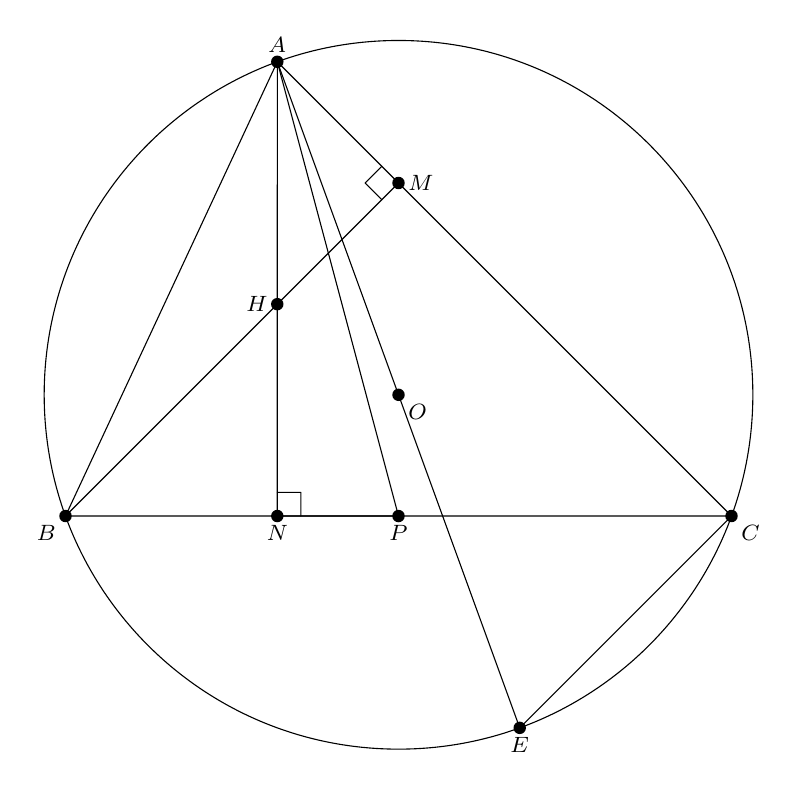
\begin{tikzpicture}[line join = round, line cap=round,>=stealth,font=\footnotesize,scale=1.5]
			\usetikzlibrary{calc,intersections,angles}
			
			% Khai báo hằng số
			\def\r{3} % r = 3cm
			
			% Định nghĩa tọa độ các điểm
			\coordinate (O) at (0,0);
			\coordinate (B) at (-160:\r); 
			\coordinate (C) at (-20:\r);  
			\coordinate (A) at (110:\r); 
			
			% N là hình chiếu của A lên BC
			\coordinate (N) at ($(B)!(A)!(C)$); % Bỏ _proj
			% M là hình chiếu của B lên AC
			\coordinate (M) at ($(A)!(B)!(C)$); % Bỏ _proj
			
			% H là giao điểm của AN và BM
			\path[name path=lineAN_H] (A) -- (N); % Sử dụng N
			\path[name path=lineBM_H] (B) -- (M); % Sử dụng M
			\path[name intersections={of=lineAN_H and lineBM_H, by=H}];
			
			% P là trung điểm của BC
			\coordinate (P) at ($(B)!0.5!(C)$);
			% Lấy điểm E sao cho O là trung điểm của AE (E = 2*O - A)
			\coordinate (E) at ($2*(O)-(A)$);
			
			% Vẽ các đối tượng hình học
			\draw (O) circle (\r);          % Đường tròn (O;r)
			\draw (A) -- (B) -- (C) -- cycle; % Tam giác A-B-C-A
			\draw (A) -- (E) -- (C);        % Đường A-E-C
			\draw (A) -- (P) -- (N) -- cycle; % Tam giác A-P-N (Sử dụng N)
			\draw (B) -- (M);            % Đoạn B-M (Sử dụng M)
			
			% Tô màu cho các điểm (theo cấu trúc đầu tiên)
			\fill (O) circle (1.5pt);
			\fill (A) circle (1.5pt);
			\fill (B) circle (1.5pt);
			\fill (C) circle (1.5pt);
			\fill (N) circle (1.5pt); % Sử dụng N
			\fill (M) circle (1.5pt); % Sử dụng M
			\fill (H) circle (1.5pt);
			\fill (P) circle (1.5pt);
			\fill (E) circle (1.5pt);
			
			% Đặt nhãn cho các điểm (theo cấu trúc đầu tiên)
			\node[below right] at (O) {$O$};
			\node[above] at (A) {$A$};
			\node[below left] at (B) {$B$};
			\node[below right] at (C) {$C$};
			\node[below] at (N) {$N$};      % Sử dụng N
			\node[right] at (M) {$M$};      % Sử dụng M
			\node[left] at (H) {$H$};      
			\node[below] at (P) {$P$};      
			\node[below] at (E) {$E$};      
			
			% Ký hiệu các góc vuông mới
			\pic[draw, angle radius=3mm]{right angle = A--N--C}; % Góc ANC (vuông tại N)
			\pic[draw, angle radius=3mm]{right angle = A--M--B}; % Góc AMB (vuông tại M)
			
		\end{tikzpicture}
		
	\end{center}
}
\end{ex}

\begin{ex} % Câu 14
	\begin{enumerate}
		\item[a)] Để tổ chức sinh nhật cho con gái, chị Linh đã đặt thợ làm bánh tại cửa hàng bánh ngọt với yêu cầu bánh được làm hai tầng, tầng phía trên cao 15cm, bán kính tầng trên là 15cm, tầng phía dưới cao 20cm đường kính tầng dưới là 40cm. Hỏi với kích thước yêu cầu của chị Linh, khi chiếc bánh được hoàn thành thì người thợ có tất cả bao nhiêu diện tích bề mặt để trang trí bánh? (mặt đáy của bánh sinh nhật không trang trí).
		\item[b)] Cho $x, y > 0$ và $x+y \le 1$.
		Tìm GTNN của biểu thức: $P = \frac{1}{x^2+y^2} + \frac{1}{xy} + 4xy$.
	\end{enumerate}
\end{ex}

\setcounterref{ex}{0}